\documentclass{beamer}

\usepackage{lmodern}

\usepackage[T2A]{fontenc}
\usepackage[utf8]{inputenc}

\usetheme{CambridgeUS}

\title[Erlang]{Исследование эффективности реализации\\некоторых структур данных на языке Erlang}
\subtitle[ПМИ]{Прикладная математика и информатика}

\author[Быцюк В.В.]{Быцюк Владислав Вячеславович}
\date[Брагилевский В.Н.]{Научный руководитель:\\старший преподаватель Брагилевский В.Н.}

\begin{document}

	% Титульный лист
	\begin{frame}
		\titlepage
	\end{frame}

	% Постановка задачи
	\begin{frame}{\LARGE \textbf{Постановка задачи}}
		\begin{itemize}
			\item Реализовать структуру данных <<упорядоченное множество>> на языке программирования Erlang.
			\item Сравнить время выполнения основных операций реализованной структуры данных с реализациями из модулей
			  	  ordsets и sets. 
		\end{itemize}
	\end{frame}
	
	
	% Основное содержание

	\begin{frame}[fragile]{\LARGE \textbf{Почему Erlang?}}
		\begin{figure}
			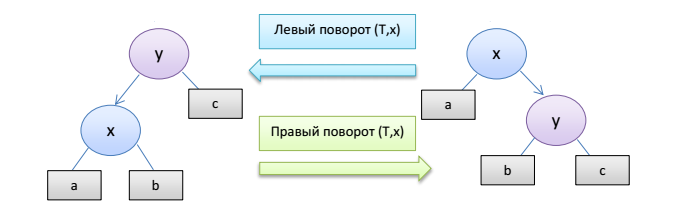
\includegraphics[scale=0.35]{img/shift.png}
		\end{figure}
		
		\begin{block}{Реализация на Erlang}
			\begin{semiverbatim}
balance(\{Key1, 
             black, 
             Left1, 
             \{Key2, red, Left2, \{Key3, red, Left3, Right3\}\}\}) ->   
	\{Key2, 
	  red, 
	  \{Key1, black, Left1, Left2\}, 
	  \{Key3, black, Left3, Right3\}\};		   
			\end{semiverbatim}
		\end{block}
	\end{frame}
	
	\begin{frame}{Сравнение времени выполнения операций вставки и удаления}
		\only<1>{\begin{figure}
			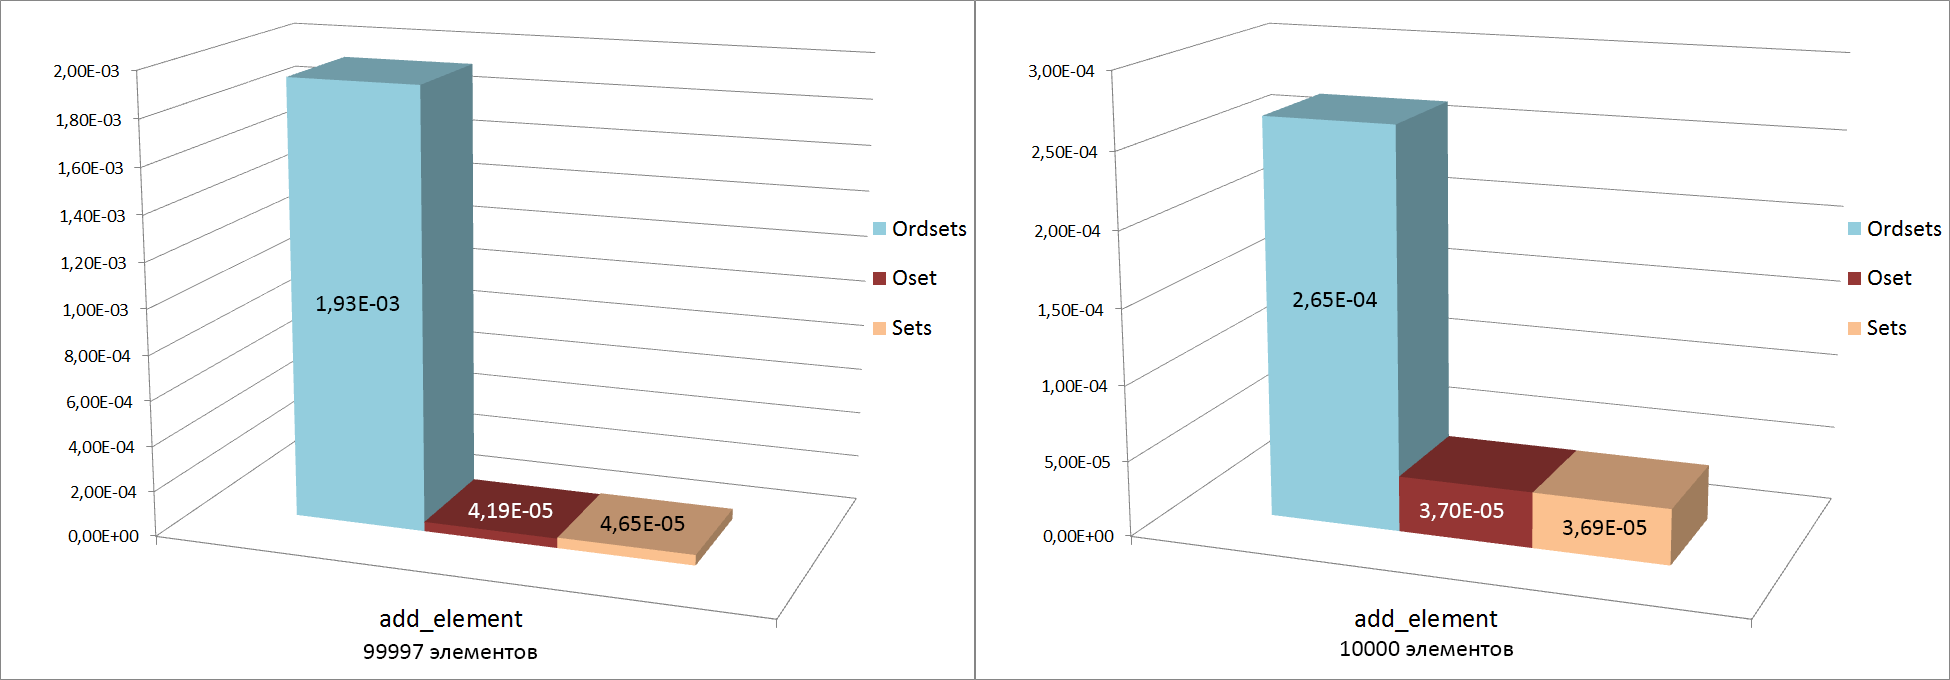
\includegraphics[scale=0.18]{img/histograms/add_element.png}
			\caption{Вставка}
		\end{figure}
		}
		\only<2>{\begin{figure}
			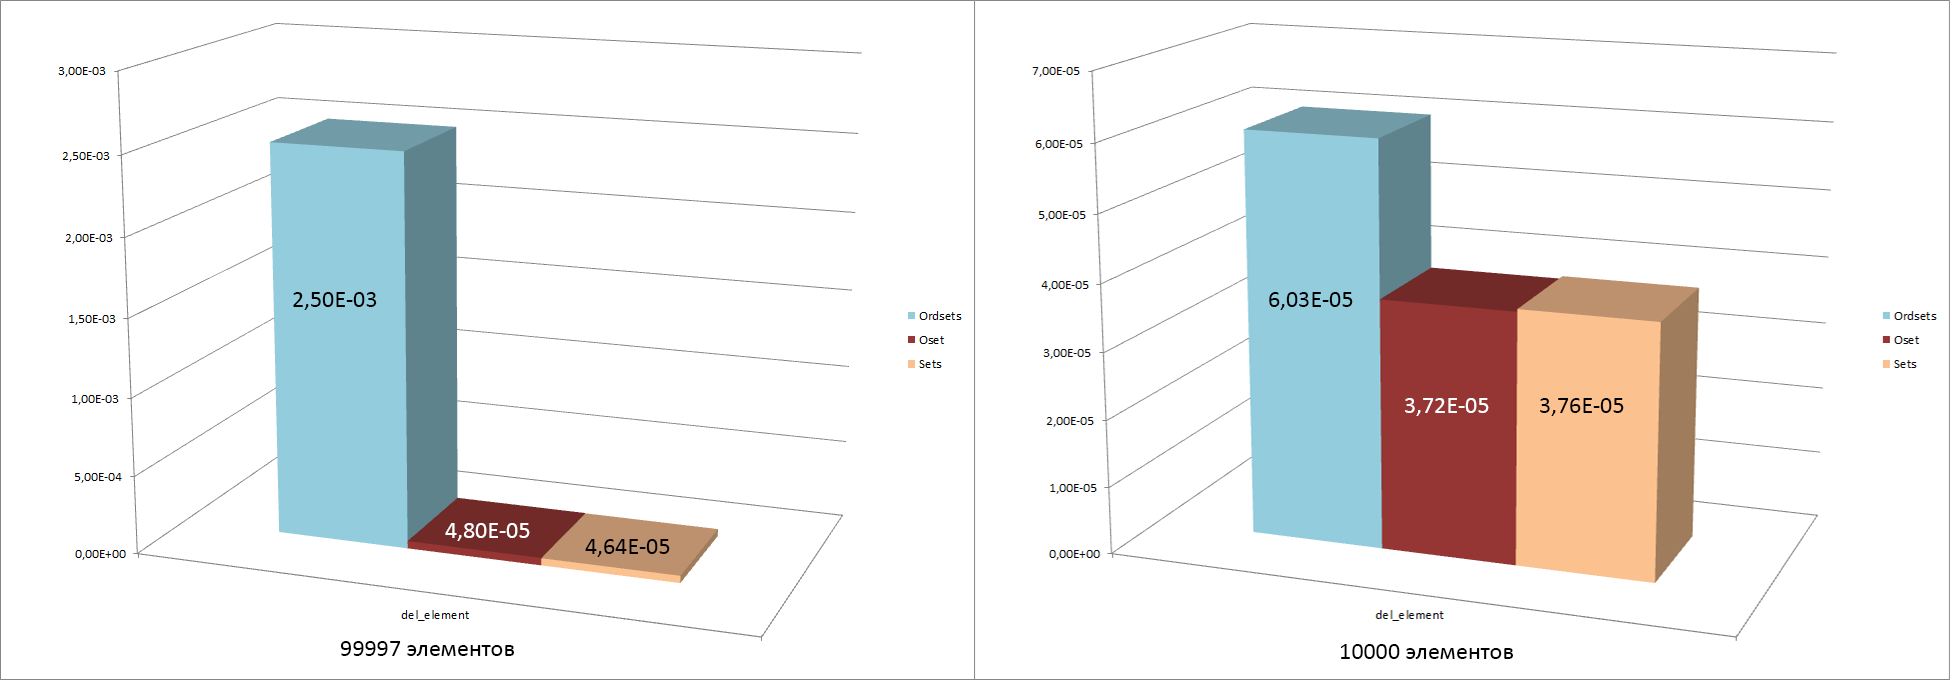
\includegraphics[scale=0.18]{img/histograms/del_element.png}
			\caption{Удаление}
		\end{figure}
		}
	\end{frame}
	
	
	\begin{frame}{Сравнение времени выполнения логических операций}
		\only<1>{\begin{figure}
			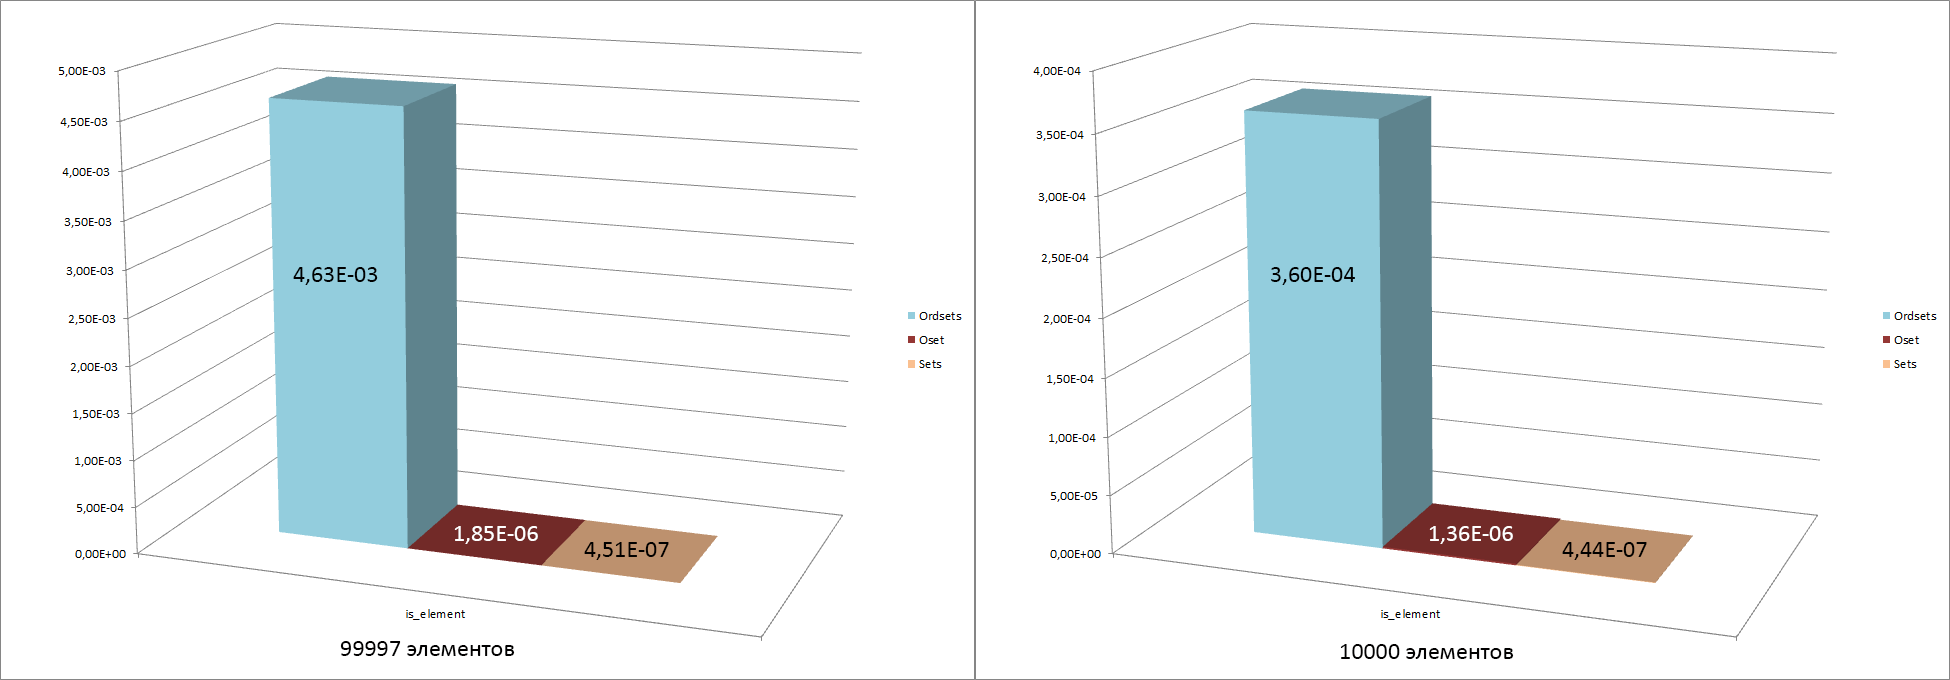
\includegraphics[scale=0.18]{img/histograms/is_element.png}
			\caption{Проверка на принадлежность элемента упорядоченному множеству}
		\end{figure}
		}
		\only<2>{\begin{figure}
			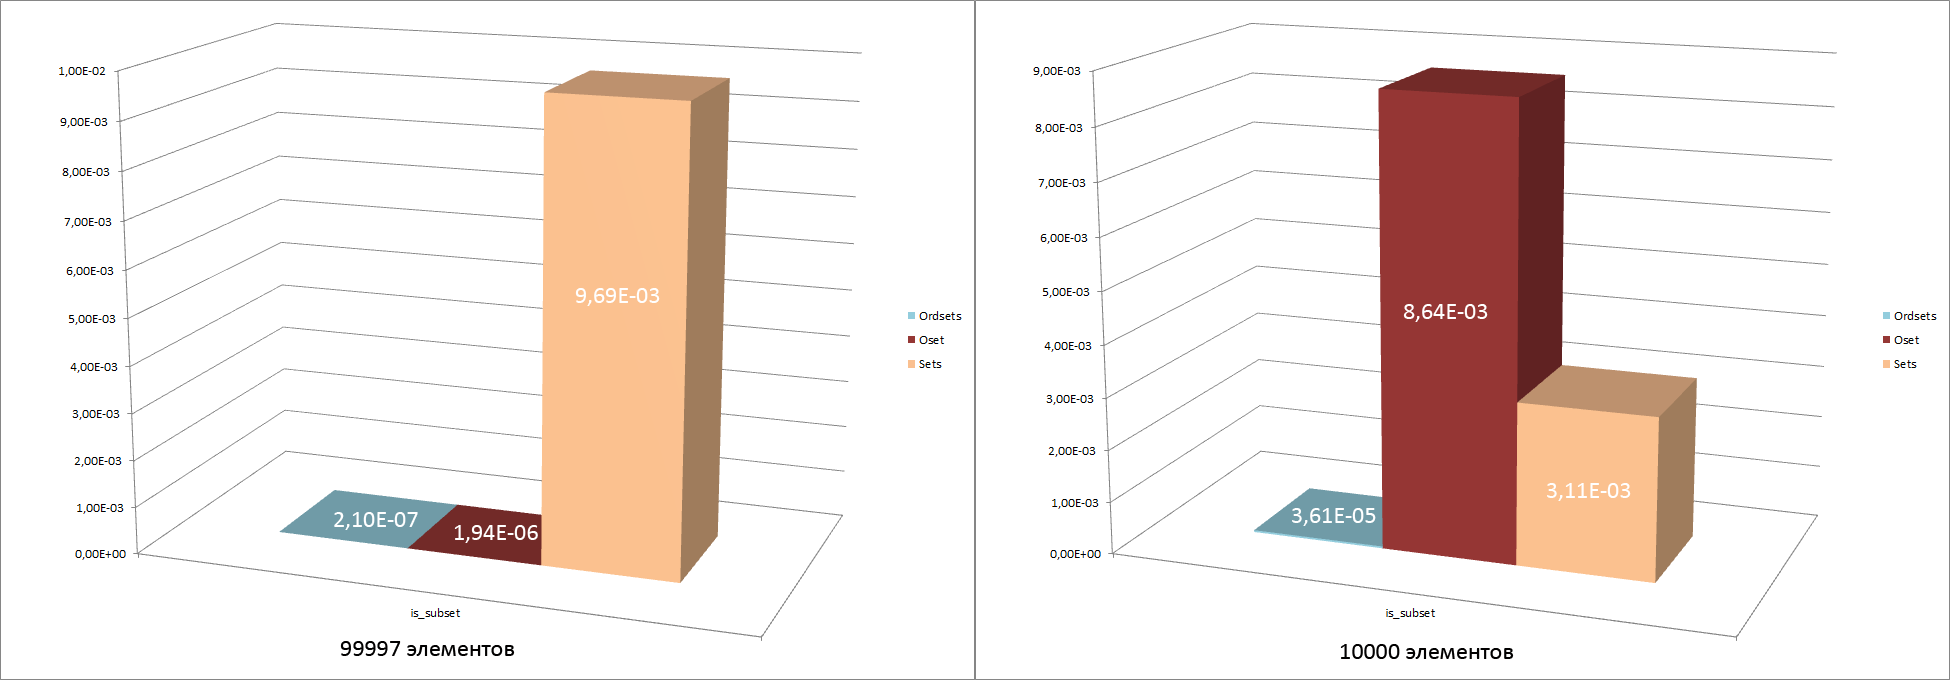
\includegraphics[scale=0.18]{img/histograms/is_subset.png}
			\caption{Проверка на то, является ли одно упорядоченное множество подмножеством другого}
		\end{figure}
		}
		\only<3>{\begin{figure}
			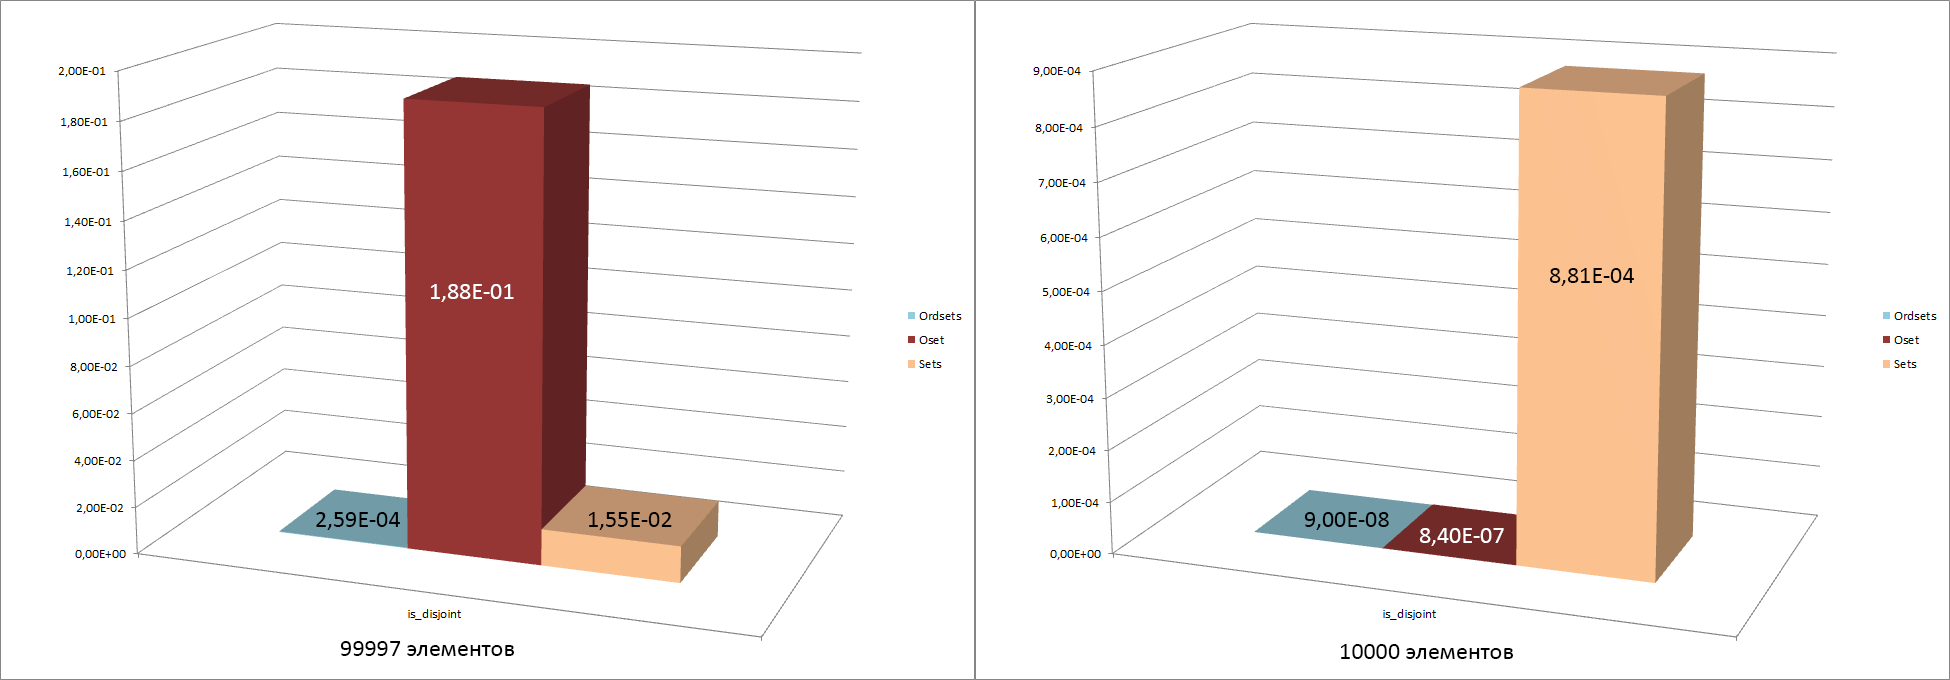
\includegraphics[scale=0.18]{img/histograms/is_disjoint.png}
			\caption{Проверка на непересекаемость двух упорядоченных множеств}
		\end{figure}
		}
	\end{frame}
	
	
	\begin{frame}{Сравнение времени выполнения перевод в список и обратно, свертки и фильтрации}
		\only<1>{\begin{figure}
			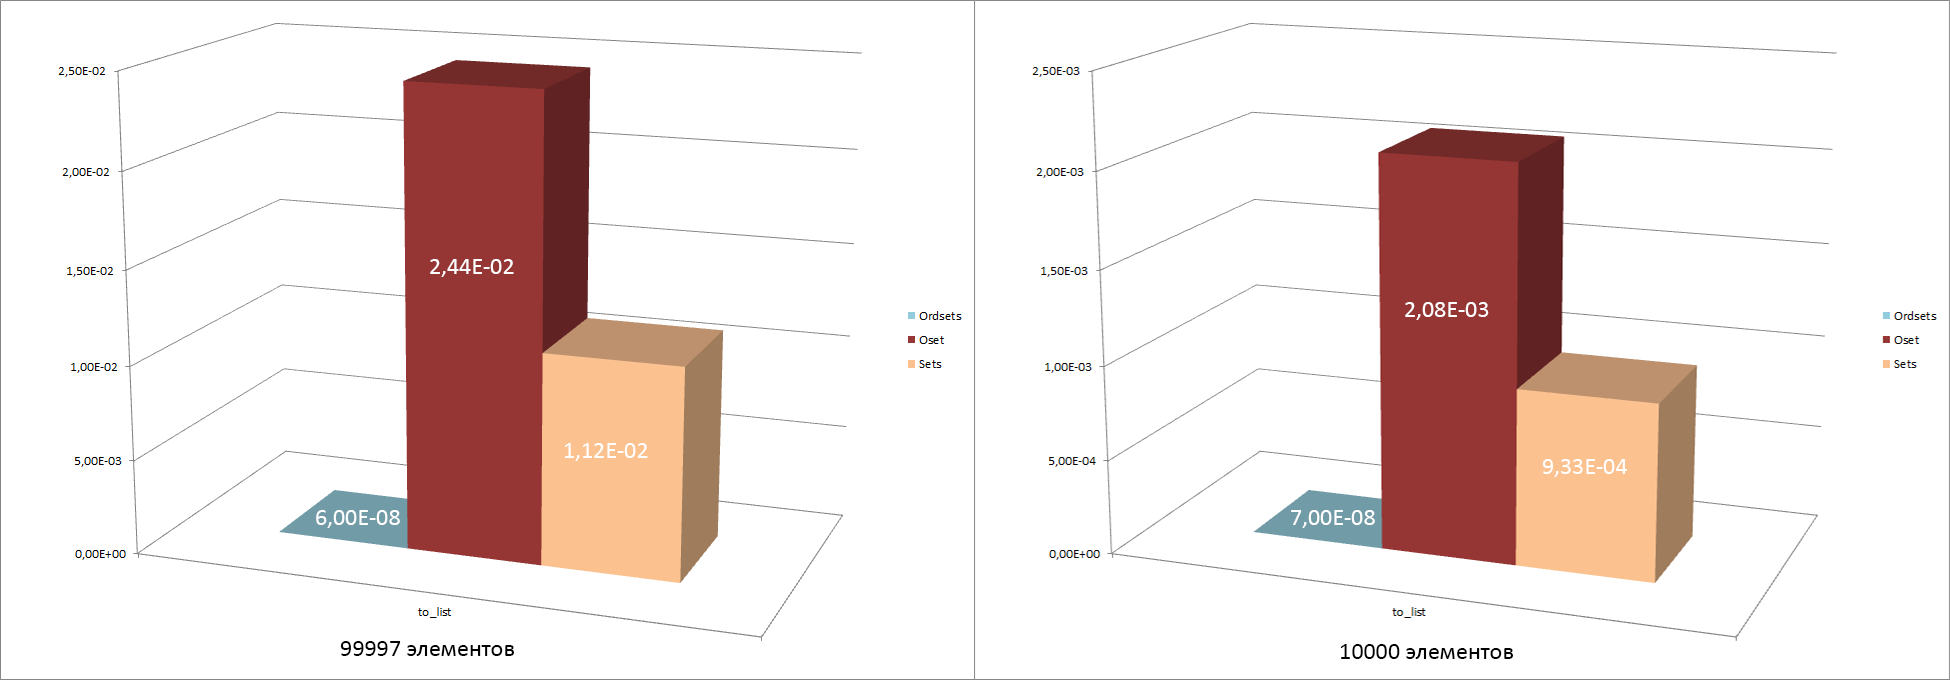
\includegraphics[scale=0.18]{img/histograms/to_list.png}
			\caption{Перевод упорядоченного множества в список}
		\end{figure}
		}
		\only<2>{\begin{figure}
			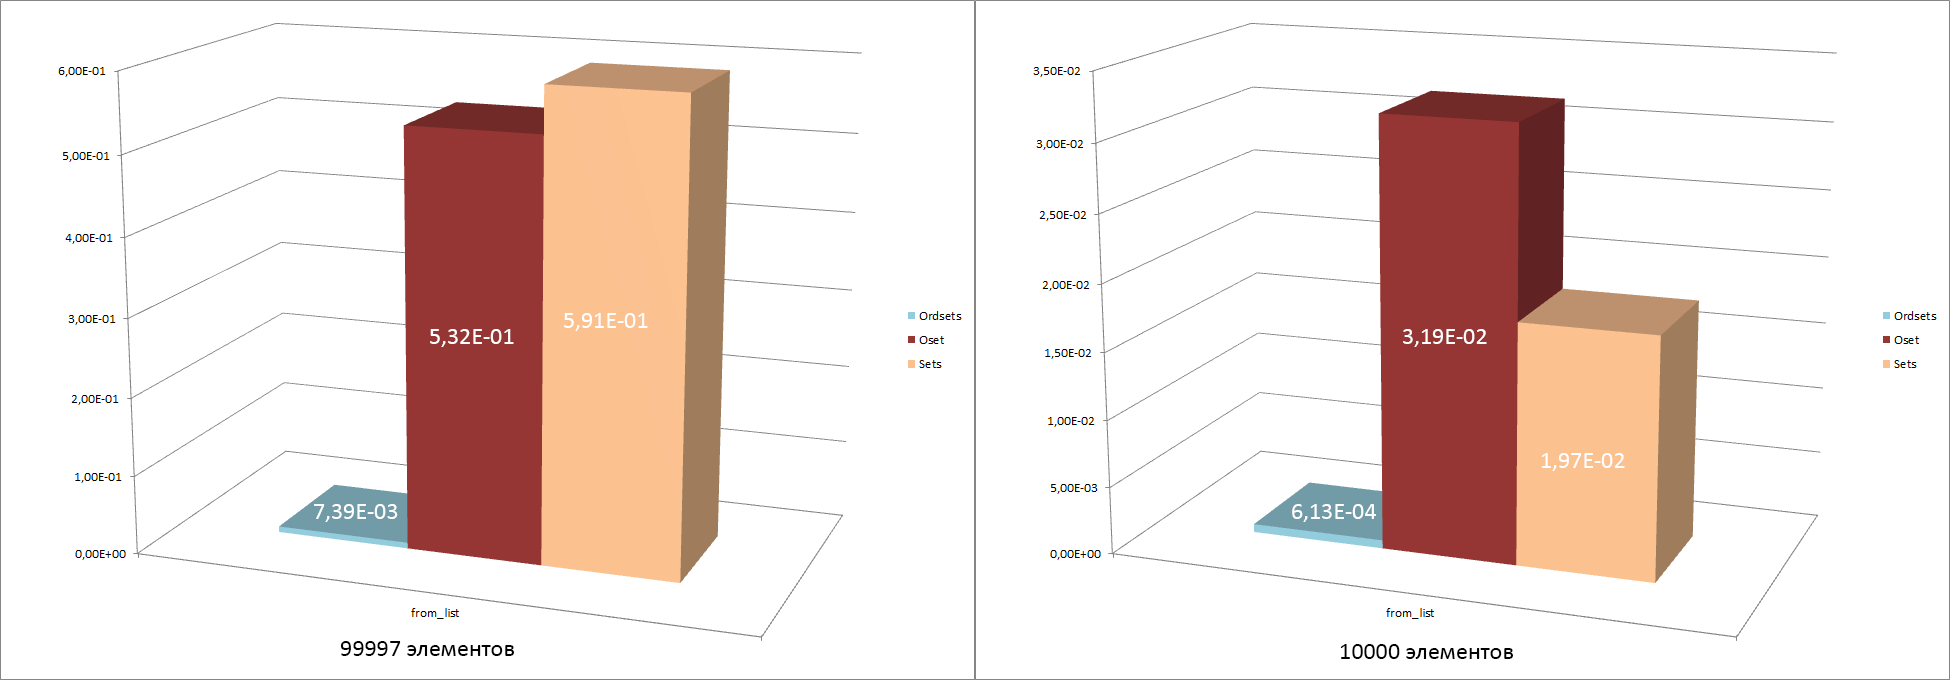
\includegraphics[scale=0.18]{img/histograms/from_list.png}
			\caption{Перевод списка в упорядоченное множество}
		\end{figure}
		}
		\only<3>{\begin{figure}
			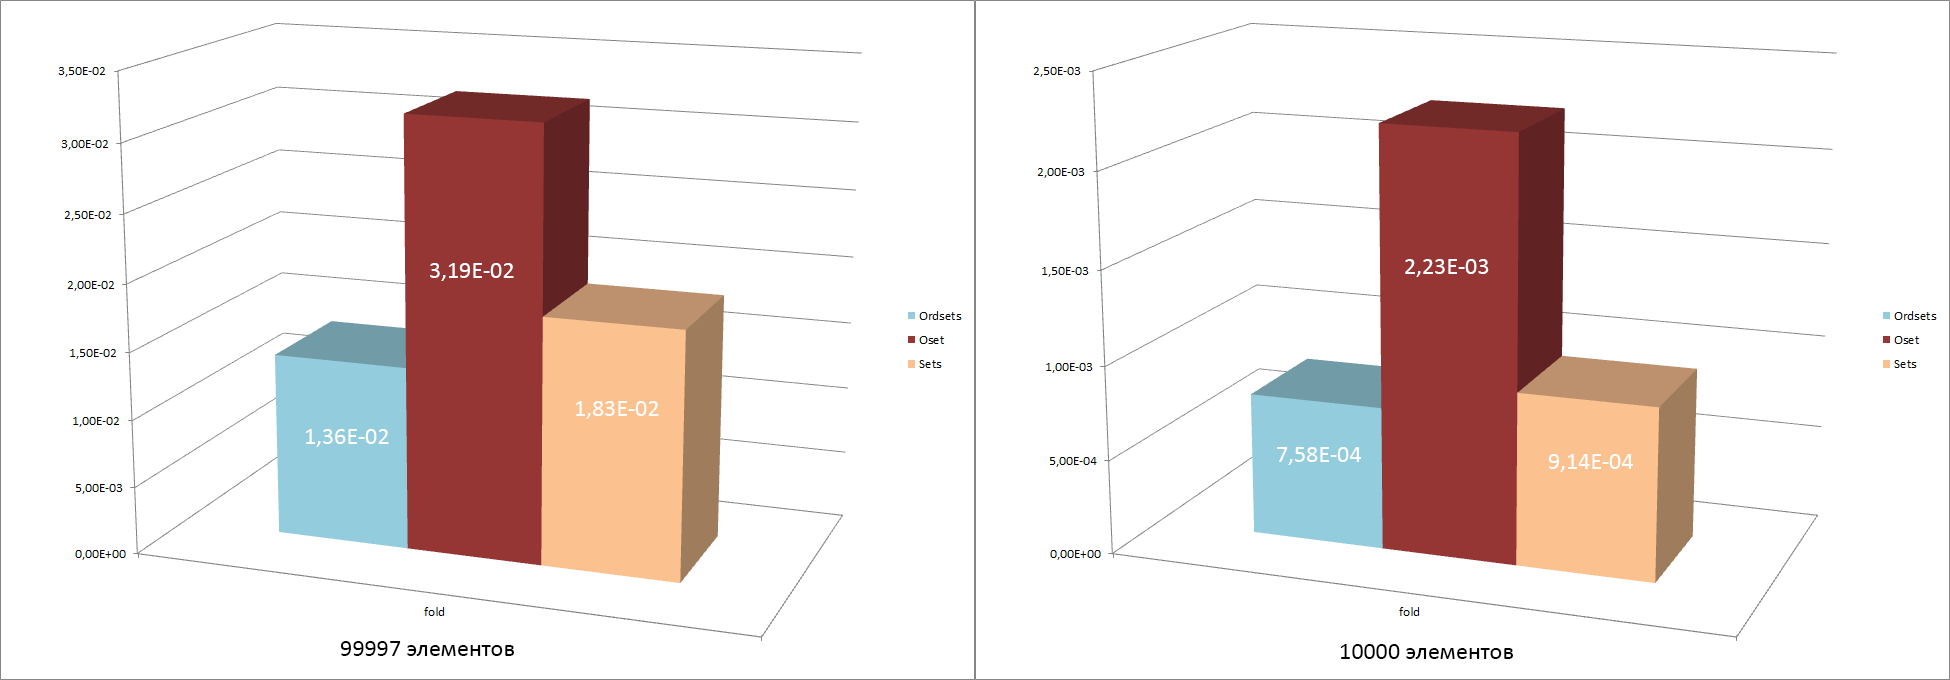
\includegraphics[scale=0.18]{img/histograms/fold.png}
			\caption{Свертка}
		\end{figure}
		}
		\only<4>{\begin{figure}
			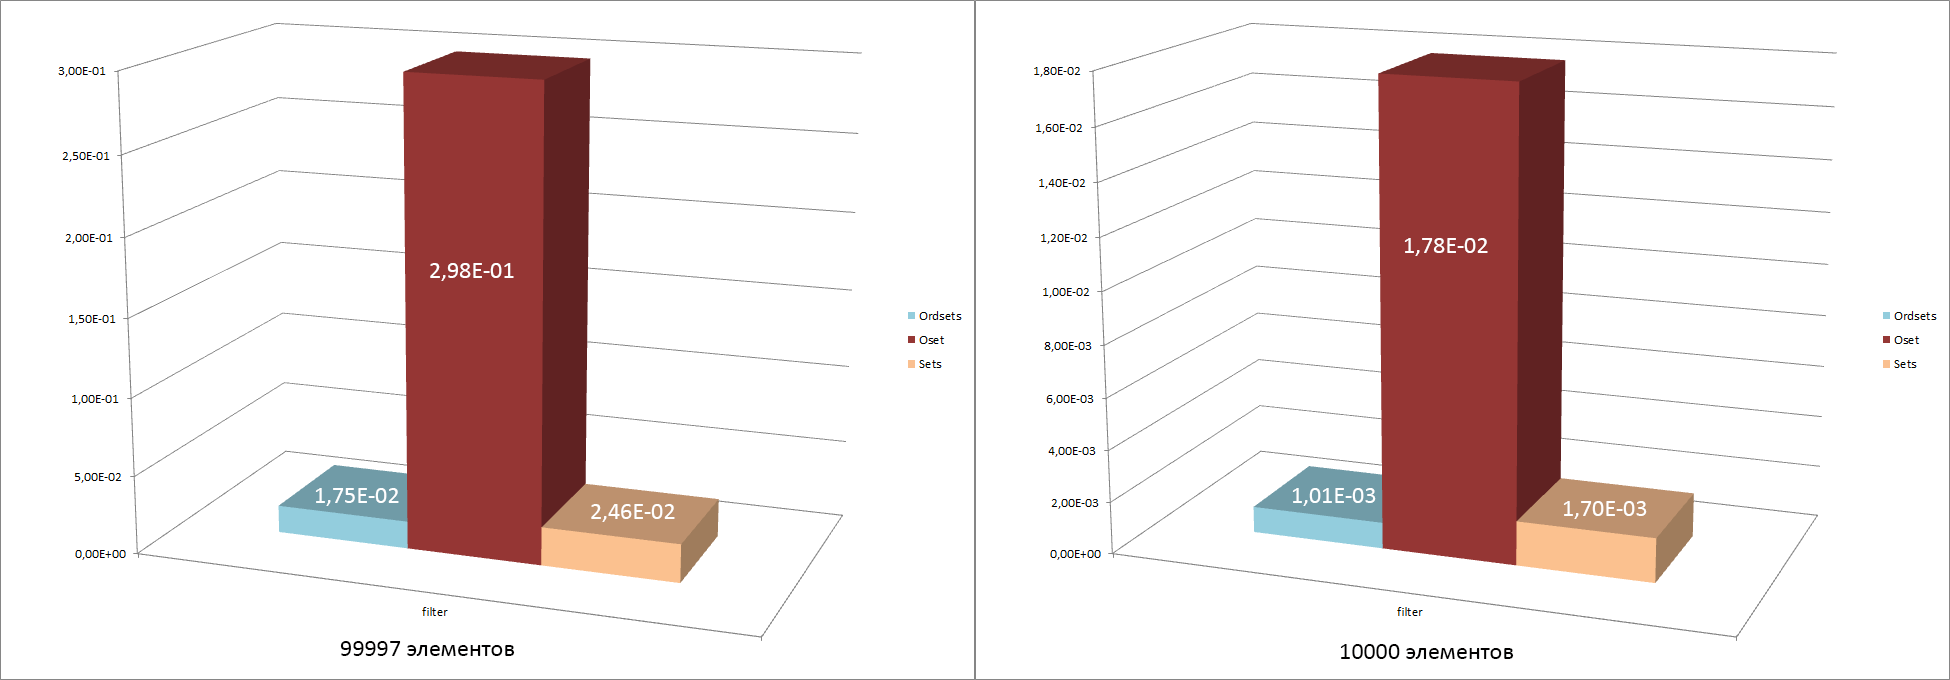
\includegraphics[scale=0.18]{img/histograms/filter.png}
			\caption{Фильтрация}
		\end{figure}
		}
	\end{frame}
	
	
	\begin{frame}{Сравнение времени выполнения операций объединения, пересечения, разности}
		\only<1>{\begin{figure}
			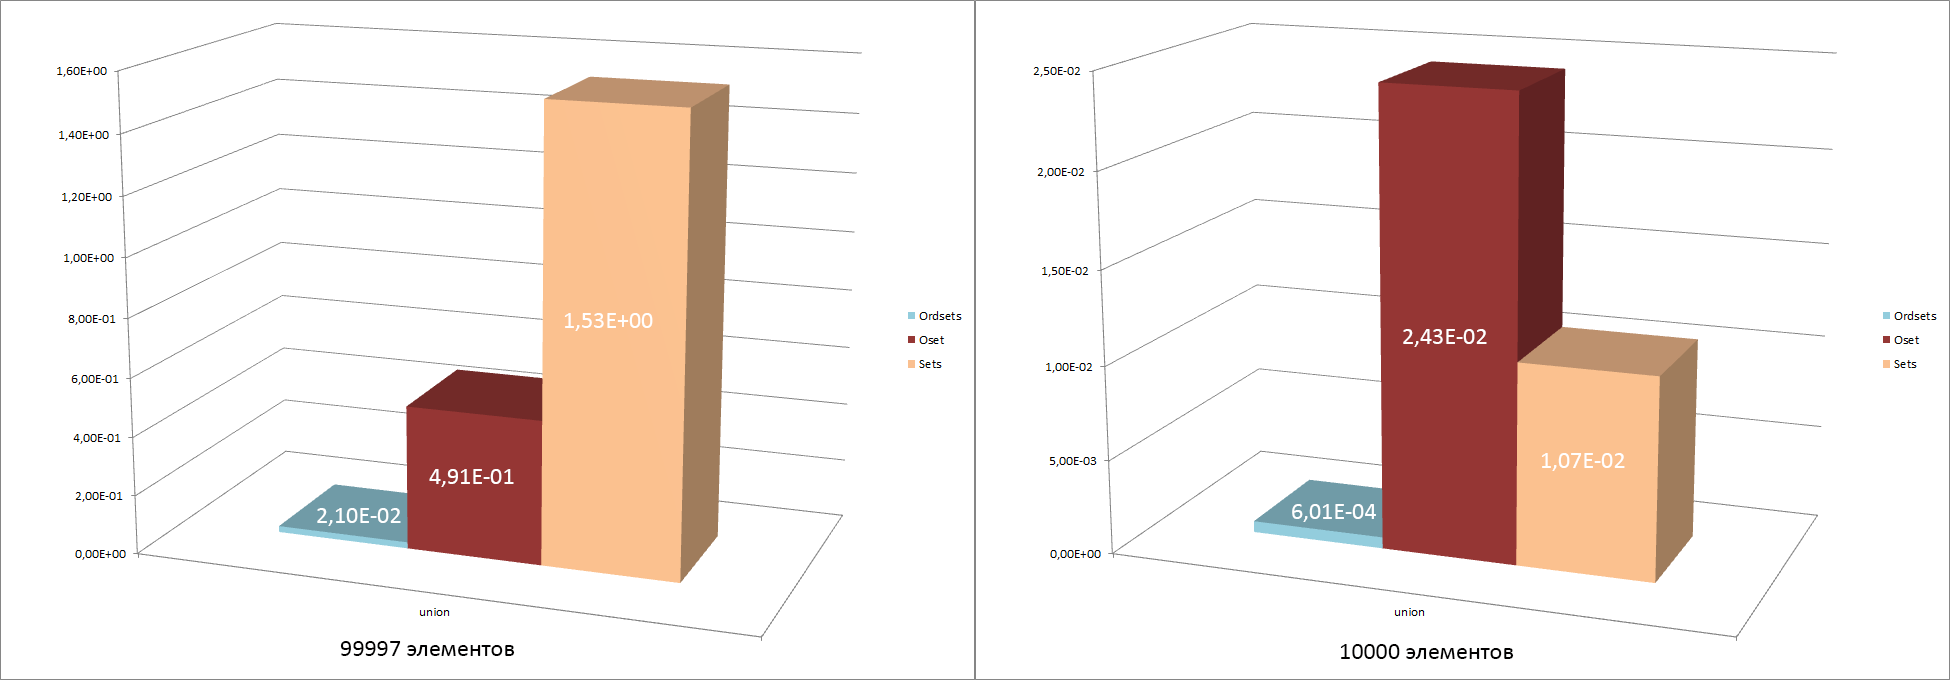
\includegraphics[scale=0.18]{img/histograms/union.png}
			\caption{Объединение}
		\end{figure}
		}
		\only<2>{\begin{figure}
			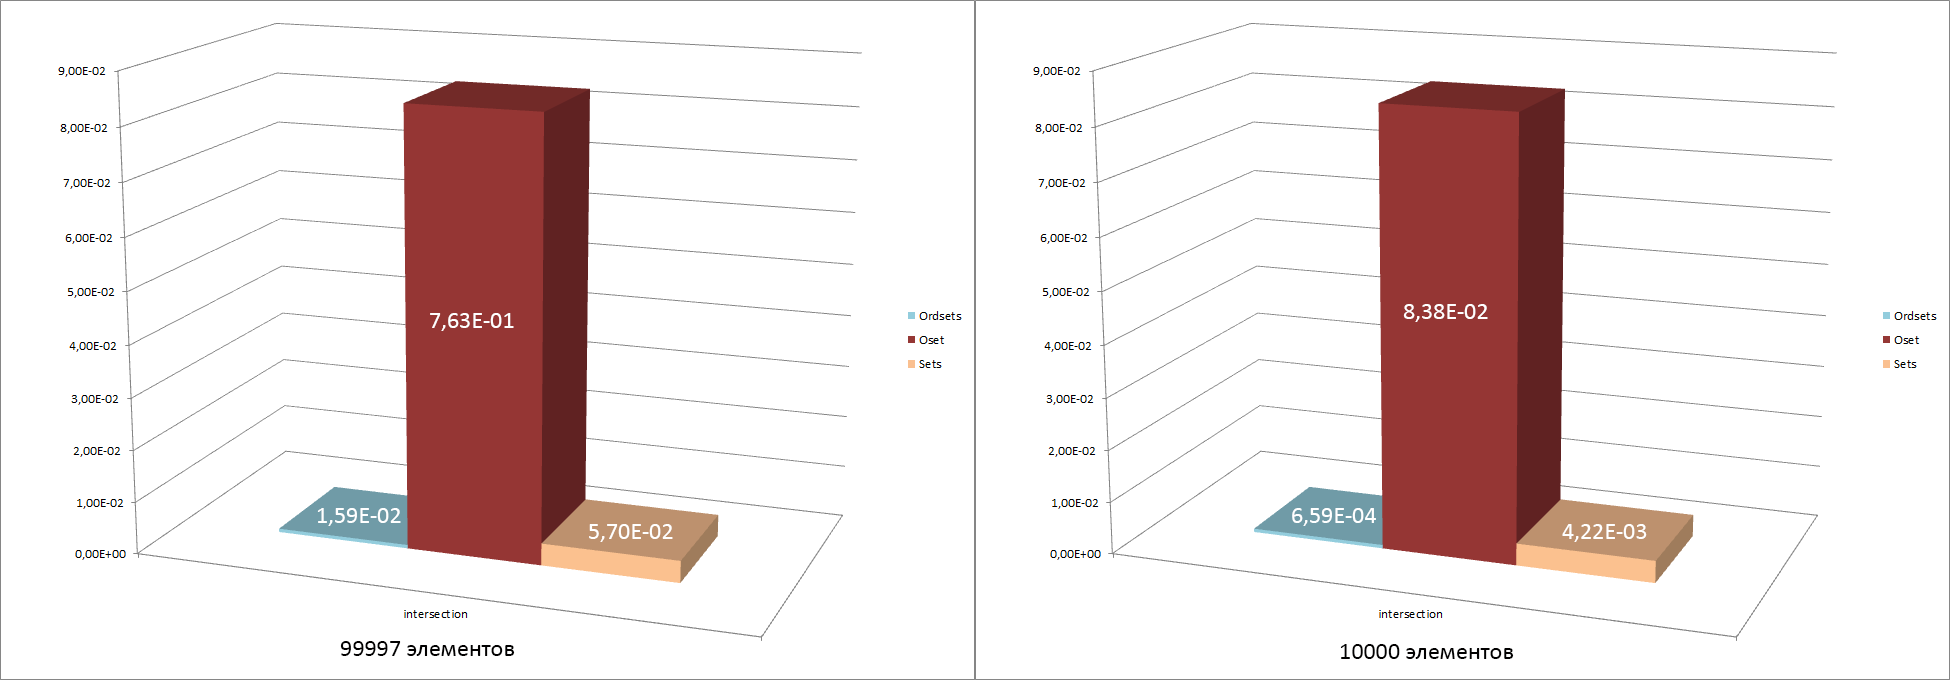
\includegraphics[scale=0.18]{img/histograms/intersection.png}
			\caption{Пересечение}
		\end{figure}
		}
		\only<3>{\begin{figure}
			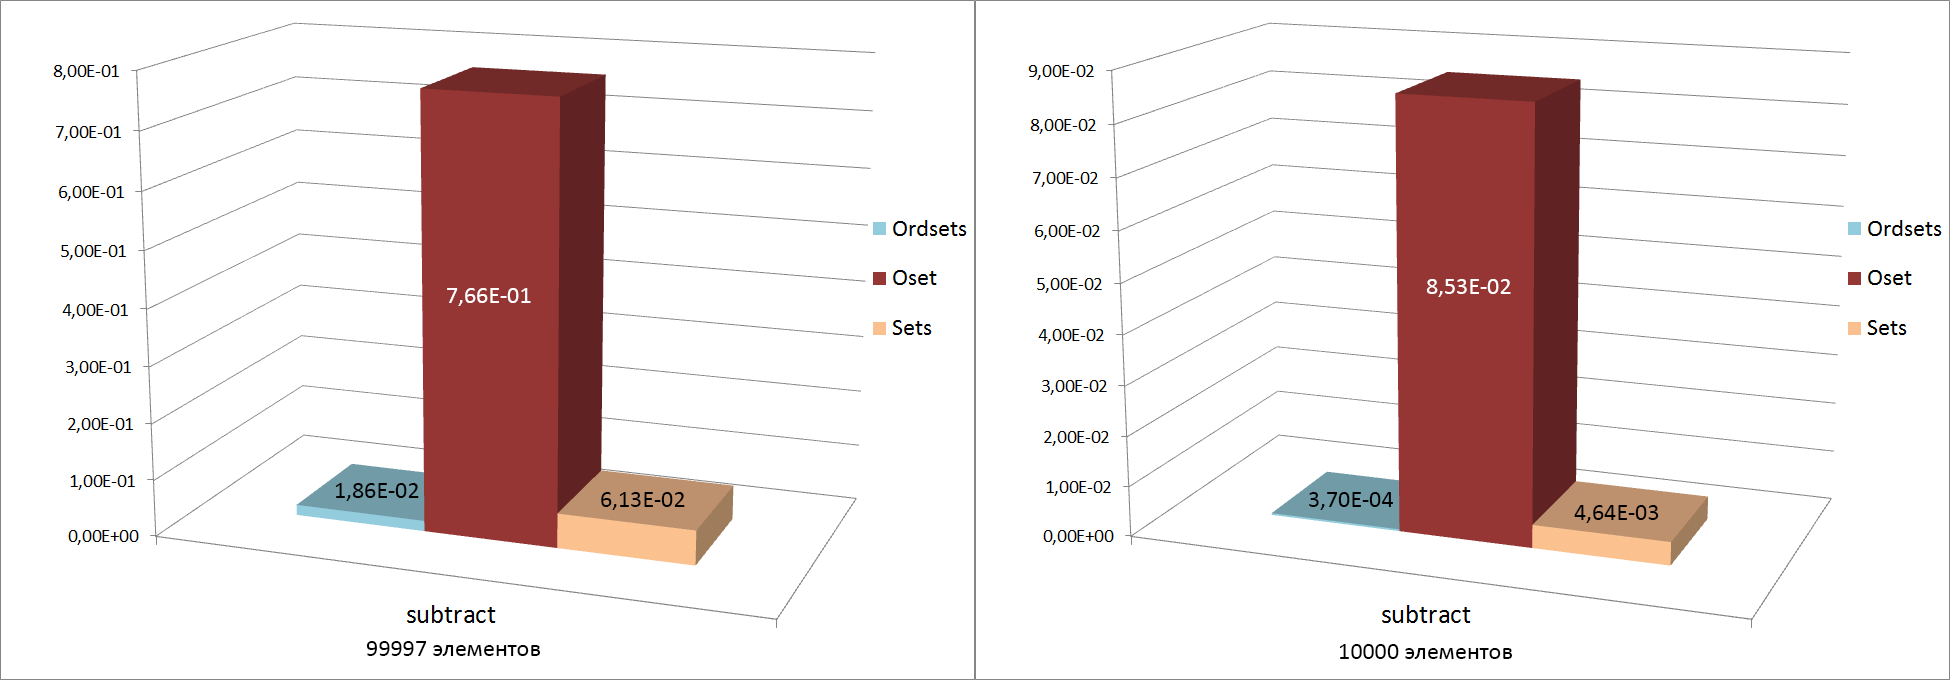
\includegraphics[scale=0.18]{img/histograms/subtract.png}
			\caption{Разность}
		\end{figure}
		}
	\end{frame}
	
	% Полученные результаты
	\begin{frame}{\LARGE \textbf{Полученные результаты}}
		\begin{itemize}
			\item Это
			\item И это
		\end{itemize}
	\end{frame}

\end{document}
